
\documentclass[twocolumn]{article}
\usepackage{mathpazo}
\usepackage{microtype}
\usepackage{times}
\usepackage{titlesec} % 1
%\usepackage{sectsty} % "제 1 절" ...

 %%%%%%%%%%%%%%%%%%%%%%%%%%%%%%%%%%%%%%%%%%%%%%%%%%%%%%%%%%%%%%%%%%%%%%%%%%%%%
 %                              My Commands
\newcommand{\bi}{\begin{itemize}}
\newcommand{\ei}{\end{itemize}}
\newcommand{\be}{\begin{enumerate}}
\newcommand{\ee}{\end{enumerate}}
\newcommand{\ii}{\item}
\newtheorem{Def}{Definition}
\newtheorem{Lem}{Lemma}
\usepackage{algorithm}
\usepackage{algorithmicx}
\usepackage{algpseudocode}

\usepackage{graphicx}
\graphicspath{%
        {converted_graphics/}
        {./images/}
}
\usepackage{hyperref}
%\usepackage[hangul,nonfrench,finemath]{kotex}
    
\setlength\textwidth{7in} 
\setlength\textheight{9.5in} 
\setlength\oddsidemargin{-0.25in} 
\setlength\topmargin{-0.25in} 
\setlength\headheight{0in} 
\setlength\headsep{0in} 
\setlength\columnsep{9pt}
\sloppy 
 
\begin{document}

\title{
\vspace{-0.5in}\rule{\textwidth}{2pt}
\begin{tabular}{ll}\begin{minipage}{4.75in}\vspace{6px}
\noindent\large {\it KIWI Project}@Data Management Research Section\\
\vspace{-12px}\\
\noindent\LARGE ETRI\qquad  \large Technical Report 14ZS1410-TR-64
\end{minipage}&\begin{minipage}{2in}\vspace{6px}\small
218 Gajeong-ro, Yuseong-gu\\
Daejeon, 305-700, South Korea\\
http:/$\!$/www.etri.re.kr/\\
http:/$\!$/sungsoo.github.com/\quad 
\end{minipage}\end{tabular}
\rule{\textwidth}{2pt}\vspace{0.25in}
\LARGE \bf Analysis of the Apache Tez Design
}

\date{}

\author{
{\bf Sung-Soo Kim}\\
\it{sungsoo@etri.re.kr}
}

\maketitle

\begin{abstract}
{\small
MapReduce has served us well. For years it has been the processing
engine for Hadoop and has been the backbone upon which a huge amount of
value has been created. While it is here to stay, new paradigms are also
needed in order to enable Hadoop to serve an even greater number of
usage patterns. A key and emerging example is the need for
\emph{interactive query}, which today is challenged by the
\emph{batch-oriented nature} of MapReduce. A key step to enabling this
new world was \emph{Apache YARN} and today the community proposes the
next step\ldots{} \emph{Tez}}
\end{abstract}

\section{Introduction}

%\begin{figure}[!t]
%        \centering
%        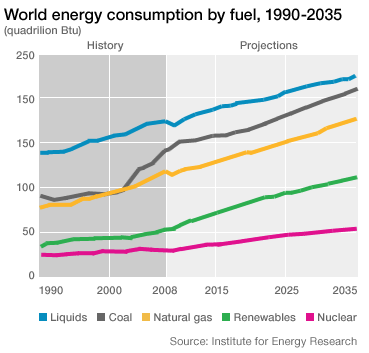
\includegraphics[width=0.33\textwidth]{test}
%        \caption{Caption}
%        \label{fig1}
%\end{figure}

\subsection{What is Tez?}

\textbf{Tez} -- Hindi for ``\emph{speed}'' provides a general-purpose, highly customizable
framework that creates simplifies data-processing tasks across both
small scale (low-latency) and large-scale (high throughput) workloads in
Hadoop. It generalizes the MapReduce paradigm to a more powerful
framework by providing the ability to execute a complex \textbf{DAG}
(\emph{directed acyclic graph}) of tasks for a single job so that
projects in the Apache Hadoop ecosystem such as Apache Hive, Apache Pig
and Cascading can meet requirements for human-interactive response times
and extreme throughput at petabyte scale (clearly MapReduce has been a
key driver in achieving this).

\subsection{What Tez Does}

Tez is the logical next step for Apache Hadoop after \textbf{Apache
Hadoop YARN}. With YARN the community generalized Hadoop MapReduce to
provide a \emph{general-purpose resource management framework} wherein
MapReduce became merely one of the applications that could process data
in a Hadoop cluster. Tez provides a more general data-processing
application to the benefit of the entire ecosystem.

Tez will speed Pig and Hive workloads by an order of magnitude. By
eliminating unnecessary tasks, synchronization barriers, and reads from
and write to HDFS, Tez speeds up data processing across both
small-scale, low-latency and large-scale, high-throughput workloads.

\begin{figure}[!t]
        \centering
        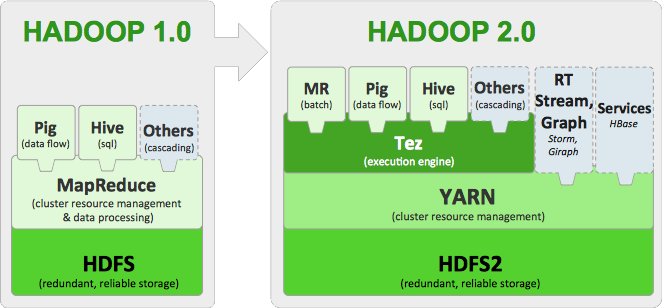
\includegraphics[width=0.48\textwidth]{hadoopstack}
        \caption{Hadoop 1.0 vs. Hadoop 2.0}
        \label{fig01}
\end{figure}

With the emergence of Apache Hadoop YARN as the basis of next generation
data-processing architectures, there is a strong need for an application
which can execute a complex DAG of tasks which can then be shared by
Apache Pig, Apache Hive, Cascading and others. The constrained DAG
expressible in MapReduce (one set of maps followed by one set of
reduces) often results in multiple MapReduce jobs which harm latency for
short queries (overhead of launching multiple jobs) and throughput for
large-scale queries (too much overhead for materializing intermediate
job outputs to the filesystem). With Tez, we introduce a more expressive
DAG of tasks, within a single application or job, that is better aligned
with the required processing task -- thus, for e.g., any \emph{given SQL
query can be expressed as a single job} using Tez.

The below graphic illustrates the advantages provided by Tez for complex
SQL queries in Apache Hive or complex Apache Pig scripts.

\begin{figure}[htb]
        \centering
        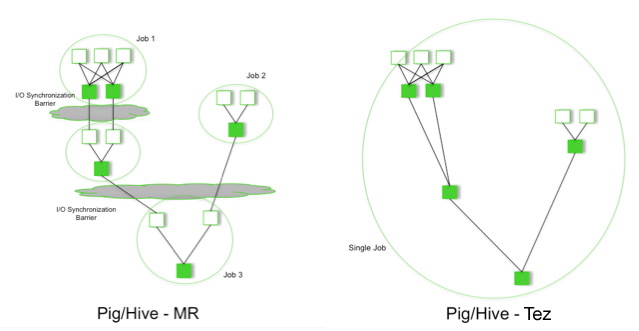
\includegraphics[width=0.48\textwidth]{pighivetez.png}
        \caption{General example of a Map-Reduce execution plan compared to DAG execution plan}
        \label{fig02}
\end{figure}

Tez is critical to the
\href{http://hortonworks.com/blog/100x-faster-hive}{\textbf{Stinger
Initiative}} and goes a long way in helping Hive support both
interactive queries and batch queries. Tez provides a single underlying
framework to support both latency and throughput sensitive applications,
there-by obviating the need for multiple frameworks and systems to be
installed, maintained and supported, a \emph{key advantage to
enterprises looking to rationalize their data architectures}.

Essentially, Tez is the logical next step for Apache Hadoop after Apache
Hadoop YARN. With YARN the community generalized Hadoop MapReduce to
provide a
\href{http://hortonworks.com/blog/introducing-apache-hadoop-yarn/}{general-purpose
resource management framework}(YARN) where-in MapReduce became merely
\emph{one of the applications} that could process data in your Hadoop
cluster. With Tez, we build on YARN and our experience with the
MapReduce to provide a more general data-processing application to the
benefit of the entire ecosystem i.e. Apache Hive, Apache Pig etc.

\subsection{Motivation}

\emph{Distributed data processing} is the core application that Apache
Hadoop is built around. Storing and analyzing \emph{large volumes} and
\emph{variety} of data efficiently has been the cornerstone use case
that has driven large scale adoption of Hadoop, and has resulted in
creating enormous value for the Hadoop adopters. Over the years, while
building and running data processing applications based on MapReduce, we
have understood a lot about the strengths and weaknesses of this
framework and how we would like to evolve the \emph{Hadoop data
processing framework} to meet the evolving needs of Hadoop users. As the
Hadoop compute platform moves into its next phase with \textbf{YARN}, it
has decoupled itself from MapReduce being the only application, and
opened the opportunity to create a new data processing framework to meet
the new challenges. Apache Tez aspires to live up to these lofty goals.

\section{Key Design Themes}

Higher-level data processing applications like Hive and Pig need an
execution framework that can express their complex query logic in an
efficient manner and then execute it with high performance. Apache Tez
has been built around the following main design themes that solve these
key challenges in the Hadoop data processing domain.

\subsection{Ability to express, model and execute data processing logic}

Tez models data processing as a \emph{dataflow graph} with vertices in
the graph representing \emph{application logic} and edges representing
\emph{movement of data}. A rich dataflow definition API allows users to
express \emph{complex query logic} in an intuitive manner and it is a
natural fit for \emph{query plans} produced by higher-level declarative
applications like \textbf{Hive} and \textbf{Pig}. As an example, the
diagram shows how to model an \emph{ordered distributed sort} using
\textbf{range partitioning}. The \emph{Preprocessor} stage sends samples
to a \textbf{Sampler} that calculates sorted data ranges for each data
partition such that the work is \emph{uniformly distributed}. The ranges
are sent to \textbf{Partition} and \textbf{Aggregate} stages that read
their assigned ranges and perform the data \emph{scatter-gather}. This
dataflow pipeline can be expressed as a single Tez job that will run the
entire computation. Expanding this logical graph into a physical graph
of tasks and executing it is taken care of by Tez.

\begin{figure}[htb]
        \centering
        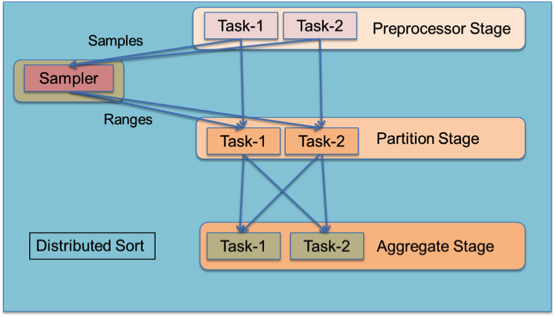
\includegraphics[width=0.48\textwidth]{tez1}
        \caption{DAG execution}
        \label{fig03}
\end{figure}

\subsection{Flexible Input-Processor-Output task model}

Tez models the user logic running in each vertex of the dataflow graph
as a composition of \textbf{Input}, \textbf{Processor} and
\textbf{Output} modules. Input \& Output determine the \emph{data
format} and how and where it is read/written. \emph{Processor} holds the
\emph{data transformation} logic. Tez does not impose any data format
and only requires that a combination of Input, Processor and Output must
be compatible with each other with respect to their formats when they
are composed to instantiate a \emph{vertex task}. Similarly, an Input
and Output pair connecting two tasks should be compatible with each
other. In the diagram, we can see how composing different Inputs,
Outputs and Processors can produce different tasks.

\begin{figure}[htb]
        \centering
        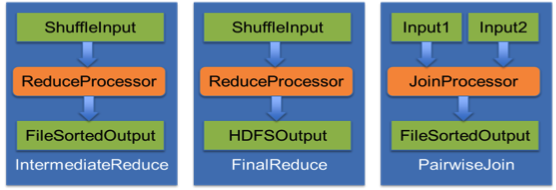
\includegraphics[width=0.48\textwidth]{tez2}
        \caption{DAG execution}
        \label{fig04}
\end{figure}

\subsection{Performance via Dynamic Graph Reconfiguration}

Distributed data processing is \emph{dynamic} by nature and it is
extremely difficult to statically determine \emph{optimal concurrency}
and \emph{data movement methods} a priori. More information is available
during runtime, like data samples and sizes, which may help optimize the
\emph{execution plan} further. We also recognize that Tez by itself
cannot always have the smarts to perform these \emph{dynamic
optimizations}. The design of Tez includes support for pluggable vertex
management modules to collect relevant information from tasks and change
the dataflow graph at runtime to optimize for performance and resource
usage. The diagram shows how Tez can determine an appropriate number of
reducers in a MapReduce like job by observing the actual data output
produced and the desired load per reduce task.

\begin{figure}[htb]
        \centering
        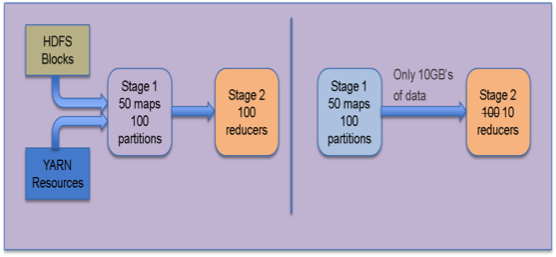
\includegraphics[width=0.48\textwidth]{tez3}
        \caption{DAG execution}
        \label{fig05}
\end{figure}

\subsection{Performance via Optimal Resource Management}

Resources acquisition in a \emph{distributed multi-tenant environment}
is based on cluster capacity, load and other quotas enforced by the
\emph{resource management framework} like \textbf{YARN}. Thus resource
available to the user may vary over time and over different executions
of the job. It becomes paramount to be able to efficiently use all
available resources to run a job as fast as possible during one instance
of execution and predictably over different instances of execution. The
Tez execution engine framework allows for efficient acquisition of
resources from YARN along with \emph{extensive reuse} of every component
in the pipeline such that no operation is duplicated unnecessarily.
These efficiencies are exposed to user logic, where possible, such that
users may also leverage this for \emph{efficient caching} and avoid
\emph{work duplication}. The diagram shows how Tez runs multiple
containers within the same YARN container host and how users can
leverage that to store their own objects that may be shared across
tasks.

\begin{figure}[htb]
        \centering
        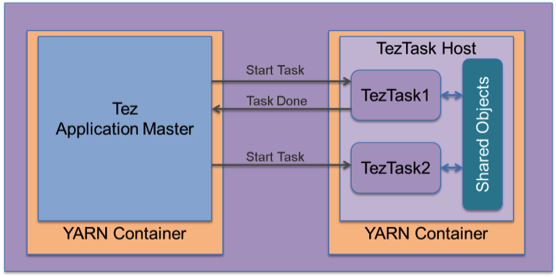
\includegraphics[width=0.48\textwidth]{tez4}
        \caption{DAG execution}
        \label{fig06}
\end{figure}


%We hope this brief overview about the philosophy and design of
%\textbf{Apache Tez} will throw some light on the aspirations of the
%project and how we hope to work with the Apache Hadoop community to
%bring them to life. \textbf{Apache Hive} and \textbf{Apache Pig}
%projects have already show deep interest in integrating with Tez.

%In the next posts in this series, we'll dive further into the
%\textbf{DAG execution} architecture, and look at MapReduce atop Tez
%along with the associated performance benefits of that model.


\section{Data Processing API in Apache Tez}
\subsection{Overview}

Apache Tez models data processing as a \emph{dataflow graph}, with the
\textbf{vertices} in the graph representing \emph{processing of data}
and \textbf{edges} representing \emph{movement of data} between the
processing. Thus \emph{user logic}, that analyses and modifies the data,
sits in the \textbf{vertices}. Edges determine the consumer of the data,
how the data is transferred and the \emph{dependency} between the
\emph{producer} and \emph{consumer} vertices. This model concisely
captures the \emph{logical definition of the computation}. When the Tez
job executes on the cluster, it expands this \emph{logical graph} into a
\emph{physical graph} by adding parallelism at the vertices to scale to
the data size being processed. Multiple tasks are created per logical
vertex to perform the computation in parallel.

\subsection{DAG Definition API}

More technically, the data processing is expressed in the form of a
\emph{directed acyclic graph} (\textbf{DAG}). The processing starts at
the root vertices of the DAG and continues down the \emph{directed
edges} till it reaches the leaf vertices. When all the vertices in the
DAG have completed then the data processing job is done. The graph does
not have cycles because the \emph{fault tolerance mechanism} used by Tez
is \textbf{re-execution} of failed tasks. When the input to a task is
lost then the producer task of the input is re-executed and so Tez needs
to be able to \emph{walk up} the graph edges to locate a non-failed task
from which to re-start the computation. \emph{Cycles} in the graph can
make this walk \emph{difficult} to perform. In some cases, cycles may be
handled by \emph{unrolling} them to create a DAG.

Tez defines a simple Java API to express a DAG of data processing. The
API has three components

\begin{itemize}
\itemsep1pt\parskip0pt\parsep0pt
\item
  \textbf{DAG.} this defines the overall job. The user creates a DAG
  object for each data processing job.\\
\item
  \textbf{Vertex.} this defines the user logic and the resources \&
  environment needed to execute the user logic. The user creates a
  Vertex object for each step in the job and adds it to the DAG.\\
\item
  \textbf{Edge.} this defines the connection between producer and
  consumer vertices. The user creates an Edge object and connects the
  producer and consumer vertices using it.
\end{itemize}

\begin{figure}[htb]
        \centering
        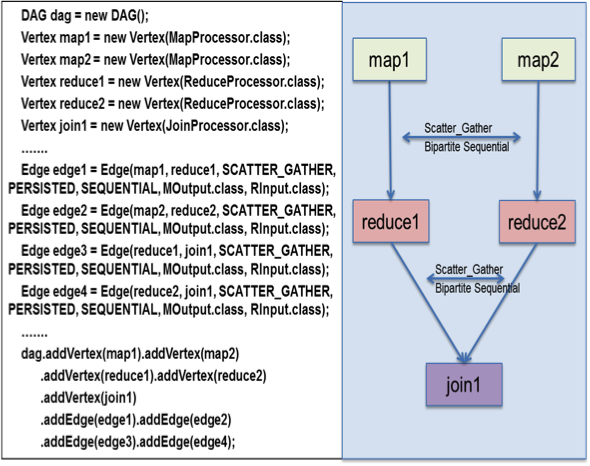
\includegraphics[width=0.48\textwidth]{tez11}
        \caption{DAG execution}
        \label{fig05}
\end{figure}

The diagram shows a \emph{dataflow graph} and its definition using the
DAG API (simplified). The job consists of 2 vertices performing a
``\textbf{Map}'' operation on 2 datasets. Their output is consumed by 2
vertices that do a ``\textbf{Reduce}'' operation. Their output is
brought together in the last vertex that does a ``\textbf{Join}''
operation.

Tez handles expanding this \emph{logical graph} at runtime to perform
the operations \emph{in parallel} using multiple tasks. The diagram
shows a runtime expansion in which the first M-R pair has a parallelism
of 2 while the second has a parallelism of 3. Both branches of
computation merge in the \textbf{Join operation} that has a parallelism
of 2. \emph{Edge properties} are at the heart of this runtime activity.

\begin{figure}[htb]
        \centering
        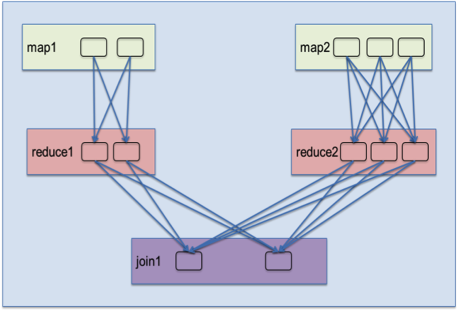
\includegraphics[width=0.48\textwidth]{tez21}
        \caption{DAG execution}
        \label{fig05}
\end{figure}


\subsection{Edge Properties}

The following edge properties enable Tez to instantiate the tasks,
configure their inputs and outputs, schedule them appropriately and help
\emph{route} the data between the tasks. The parallelism for each vertex
is determined based on \emph{user guidance}, \emph{data size} and
\emph{resources}.

\begin{itemize}
\itemsep1pt\parskip0pt\parsep0pt
\item
  \textbf{Data movement.} Defines \emph{routing} of data between tasks\\

  \begin{itemize}
  \itemsep1pt\parskip0pt\parsep0pt
  \item
    \emph{One-To-One}: Data from the \emph{i}th producer task routes to
    the \emph{i}th consumer task.\\
  \item
    \emph{Broadcast}: Data from a producer task routes to \emph{all}
    consumer tasks.\\
  \item
    \emph{Scatter-Gather}: Producer tasks \emph{scatter} data into
    \emph{shards} and consumer tasks \emph{gather} the \emph{shards}.
    The \emph{i}th shard from all producer tasks routes to the
    \emph{i}th consumer task.\\
  \end{itemize}
\item
  \textbf{Scheduling.} Defines when a \emph{consumer} task is
  scheduled\\

  \begin{itemize}
  \itemsep1pt\parskip0pt\parsep0pt
  \item
    \emph{Sequential}: Consumer task may be scheduled after a
    \emph{producer task} completes.\\
  \item
    \emph{Concurrent}: Consumer task must be \emph{co-scheduled} with a
    producer task.\\
  \end{itemize}
\item
  \textbf{Data source.} Defines the \emph{lifetime}/\emph{reliability}
  of a task output\\

  \begin{itemize}
  \itemsep1pt\parskip0pt\parsep0pt
  \item
    \emph{Persisted}: Output will be available after the task exits.
    Output may be lost later on.
  \item
    \emph{Persisted-Reliable}: Output is reliably stored and will always
    be available\\
  \item
    \emph{Ephemeral}: Output is available only while the producer task
    is running
  \end{itemize}
\end{itemize}

\begin{figure}[htb]
        \centering
        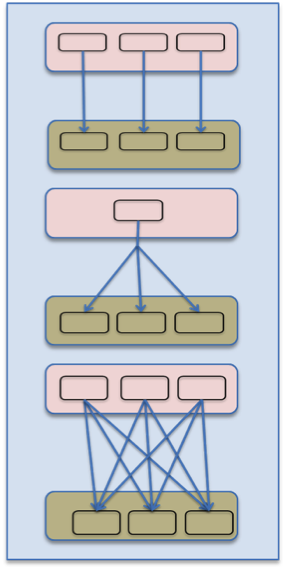
\includegraphics[width=0.48\textwidth]{tez31}
        \caption{DAG execution}
        \label{fig05}
\end{figure}

Some real life use cases will help in clarifying the edge properties.
\textbf{Mapreduce} would be expressed with the \emph{scatter-gather},
\emph{sequential} and \emph{persisted} edge properties. \textbf{Map
tasks} \emph{scatter} partitions and reduce tasks gather them.
\textbf{Reduce tasks} are \emph{scheduled} after the map tasks complete
and the map task outputs are written to local disk and hence available
after the map tasks have completed. When a vertex \emph{checkpoints} its
output into HDFS then its \emph{output edge} has a
\emph{persisted-reliable} property. If a producer vertex is
\emph{streaming data} directly to a consumer vertex then the edge
between them has \emph{ephemeral} and \emph{concurrent} properties. A
\emph{broadcast} property is used on a \emph{sampler vertex} that
produces a \textbf{global histogram} of data ranges for \emph{range
partitioning}.

We hope that the Tez dataflow definition API will be able to express a
broad spectrum of \emph{data processing topologies} and enable higher
level languages to elegantly transform their queries into Tez jobs.















\end{document}
